%%%%%%%%%%%%%%%%%%%%%%%%%%%%%%%%%%%%%%%%%%%%%%%%%%%%%%%%%%%%%%%%%%%%%%%%%%
%% FACTORING
%%%%%%%%%%%%%%%%%%%%%%%%%%%%%%%%%%%%%%%%%%%%%%%%%%%%%%%%%%%%%%%%%%%%%%%%%%

\chapter{Factoring Primes}\label{ch:factoring_primes}

Let $p$ be a prime and $\sO_K$ the ring of integers of a number field.
This chapter is about how to write $p\sO_K$ as a product of prime ideals
of $\sO_K$. Paradoxically, computing the explicit prime ideal factorization
of $p\sO_K$ is easier than computing~$\sO_K$.

%Ideals were introduced to mathematics by Kummer long ago because in
%rings of integers of number fields, ideals factor uniquely as products
%of primes ideals, despite the fact that algebraic integers need not
%factor uniquely as products of irreducible algebraic integers.  This
%failure of unique factorization for algebraic integers was used by
%Liouville to refute Lam\'{e}'s purported 1847 proof of Fermat's
%Last Theorem.

%(Recall that by Theorem~\ref{thm:uniqfac},
%such a product representation is unique.)

%Then I will sketch the main results and definitions
%that we will study in detail during the next few chapters.  We will
%cover discriminants and norms of ideals, define the class group of
%$\sO_K$ and prove that it is finite and computable, and define the
%group of units of $\sO_K$, determine its structure, and prove that it
%is also computable.

\section{The Problem}

\begin{figure}
  \centering
  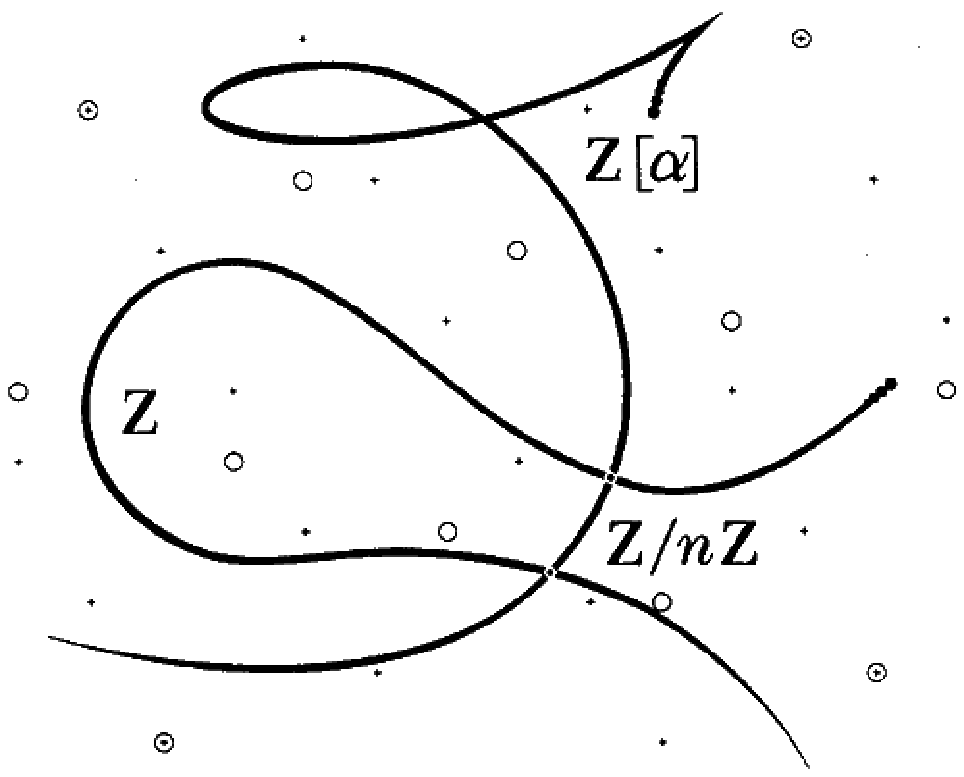
\includegraphics[width=20em]{img/spec}
  \caption{A diagram from \cite{lenstras:nfs}}.
\end{figure}

\todo{INSERT PICTURE}
%\begin{center}
%\begin{minipage}{0.7\linewidth}
%``The obvious mathematical breakthrough would be development of an easy
%way to factor large prime numbers.''
%
%-- {Bill Gates, {\em The Road Ahead}, 1st ed., pg 265}
%\end{minipage}
%\begin{minipage}{0.2\linewidth}
%
\includegraphics[width=1in]{img/Bill_Gates_June_2015}
%https://commons.wikimedia.org/wiki/File:Bill_Gates_June_2015.jpg
%\end{center}

Bill Gates meant\footnote{This quote is on page 265 of the first
  edition.  In the second edition, on page 303, this sentence is
  changed to ``The obvious mathematical breakthrough that would defeat
  our public key encryption would be the development of an easy way to
  factor large numbers.''  This is less nonsensical; however, fast
  factoring is {\em not} known to break all commonly used public-key
  cryptosystem.  For example, there are cryptosystems based on the
  difficulty of computing discrete logarithms in $\FF_p^*$ and on
  elliptic curves over $\FF_p$, which (presumably) would not be broken
  even if one could factor large numbers quickly.}  factoring products
of two primes, which would break the RSA cryptosystem (see
e.g. \cite[\S3.2]{stein:ent}).  However, perhaps Gates is an
algebraic number theorist, and he really meant what he said: then we
might imagine that he meant factorization of primes of~$\ZZ$ in rings
of integers of number fields.  For example, $2^{16}+1 = 65537$ is a
``large'' prime, and in $\ZZ[i]$ we have
$$
  (65537) = (65537, 2^8 + i) \cdot (65537, 2^8 - i).
$$

\subsection{Geometric Intuition}\label{sec:geom_intuition}

Let $K=\QQ(\alpha)$ be a number field, and let $\sO_K$ be the ring of integers
of $K$. To employ our geometric intuition, as the Lenstras did on the cover
of \cite{lenstras:nfs}, it is helpful to view $\sO_K$ as a 1-dimensional scheme
$$
  X = \Spec(\sO_K) = \{\text{all prime ideals of $\sO_K$}\}
$$
over
$$
  Y=\Spec(\ZZ) = \{ (0) \} \cup \{ p\ZZ : p \in\ZZ_{>0} \text{ is prime}\}.
$$
There is a natural map $\pi: X \rightarrow Y$ that sends a prime ideal $\p\in X$ to
$\p \cap \ZZ\in Y$. For example, if
$$
  \p = (65537, 2^8 + i) \subset \ZZ[i],
$$
then $\p \cap \ZZ = (65537)$. For more on this viewpoint,
see \cite{hartshorne} and \cite[Ch.~2]{eisenbud_harris:geometry}.

If $p\in\ZZ$ is a prime number, then the ideal $p\sO_K$ of $\sO_K$
factors uniquely as a product $\prod \p_i^{e_i}$, where the $\p_i$ are
maximal ideals of $\sO_K$.  We may imagine the decomposition of $p\sO_K$
into prime ideals geometrically as the fiber $\pi^{-1}(p\ZZ)$, where
the exponents $e_i$ are the multiplicities of the fibers.  Notice that
the elements of $\pi^{-1}(p\ZZ)$ are the prime ideals of $\sO_K$ that
contain~$p$, i.e., the primes that divide $p\sO_K$.
This chapter is about how to compute the $\p_i$ and $e_i$.

\begin{remark}
  More technically, in algebraic geometry one defines the inverse
  image of the point $p\ZZ$ to be the spectrum of the tensor product
  $\sO_K \otimes_{\ZZ} \ZZ/\p\ZZ$; by a generalization of the Chinese
  Remainder Theorem, we have
  $$
    \sO_K \otimes_{\ZZ} \left(\ZZ/\p\ZZ\right) \isom \bigoplus \sO_K/\p_i^{e_i}.
  $$
\end{remark}

\begin{exercise}
  Let $L/K$ be an extension of number fields. Let $\p$ be a prime of $K$.
  Show that the factorization of the ideal $\p\sO_L$ contains exactly the primes
  of $\sO_L$ that lay over $\p$. That is, a prime $\q$ of $\sO_L$ appears in
  the factorization of $\p\sO_L$ if and only if $\q \cap \sO_K = \p$.
\end{exercise}

\begin{exercise}
  Let $\varphi: R \to S$ be a homomorphism of (commutative) rings.
  \begin{enumerate}
    \item Prove that if $I \subset S$ is an ideal, then $\varphi^{-1}(I)$
    is an ideal of~$R$.
    \item Prove moreover that if $I$ is prime, then $\varphi^{-1}(I)$ is
    also prime.
  \end{enumerate}
\end{exercise}

\begin{exercise}
  Let $\sO_K$ be the ring of integers of a number field.
  The \defn{Zariski topology} on the set $X=\Spec(\sO_K)$ of all prime ideals
  of $\sO_K$ has closed sets the sets of the form
  $$
    V(I) = \{ \p\in X : \p \mid I\},
  $$
  where~$I$ varies through {\em all} ideals of $\sO_K$, and $\p\mid I$ means
  that $I \subset \p$.
  \begin{enumerate}
    \item\label{exercise:zariski-part-1} Prove that the collection of closed
    sets of the form $V(I)$ is a topology on $X$.
    \item Let $Y$ be the subset of nonzero prime ideals of $\sO_K$, with the
    induced topology. Use unique factorization of ideals to prove that the
    closed subsets of~$Y$ are exactly the finite subsets of~$Y$ along with
    the set~$Y$.
    \item Prove that the conclusion of the first part is still true
    if $\sO_K$ is replaced by an order in $\sO_K$, i.e., a subring that
    has finite index in $\sO_K$ as a $\ZZ$-module.
  \end{enumerate}
\end{exercise}

\begin{exercise}
  Let $\sO_K$ be the ring of integers of a number field $K$, and let $p\in\ZZ$
  be a prime number. What is the cardinality of $\sO_K/(p)$ in terms of $p$
  and $[K:\QQ]$, where $(p)$ is the ideal of $\sO_K$ generated by~$p$?
\end{exercise}

\begin{exercise}
  Which of the following rings have infinitely many prime ideals?
  \begin{enumerate}
    \item[(a)]
    The integers $\ZZ$.
    \item[(b)]
    The ring $\ZZ[x]$ of polynomials over $\ZZ$.
    \item[(c)]
    The quotient ring $\CC[x]/(x^{2005}-1)$.
    \item[(d)]
    The ring $(\ZZ/6\ZZ)[x]$ of polynomials over the ring $\ZZ/6\ZZ$.
    \item[(e)]
    The quotient ring $\ZZ/n\ZZ$, for a fixed positive integer~$n$.
    \item[(f)]
    The rational numbers~$\QQ$.
    \item[(g)]
    The polynomial ring $\QQ[x,y,z]$ in three variables.
  \end{enumerate}
\end{exercise}

\subsection{Examples}

The following {\Sage} session shows the commands needed to compute
the factorization of $p\sO_K$ for~$K$ the number field defined by
a root of $x^5 + 7x^4 + 3x^2 - x + 1$ and $p = 2$ and~$5$. We first
create an element $f\in \QQ[x]$ in {\Sage}:
\begin{sagecode}
\begin{sagecell}
R.<x> = QQ[]
f = x^5 + 7*x^4 + 3*x^2 - x + 1
\end{sagecell}
\end{sagecode} %link

\noindent
Then we create the corresponding number field obtained
by adjoining a root of $f$, and find its ring of integers.
%link
\begin{sagecode}
\begin{sagecell}
K.<a> = NumberField(f)
OK = K.ring_of_integers()
OK.basis()
\end{sagecell}
\begin{sageout}
[1, a, a^2, a^3, a^4]
\end{sageout}
\end{sagecode} %link

\noindent
We define the ideal $2\sO_K$ and factor -- it turns out to be prime.

%link
\begin{sagecode}
\begin{sagecell}
I = K.fractional_ideal(2); I
\end{sagecell}
\begin{sageout}
Fractional ideal (2)
\end{sageout}
\begin{sagecell}
I.factor()
\end{sagecell}
\begin{sageout}
Fractional ideal (2)
\end{sageout}
\begin{sagecell}
I.is_prime()
\end{sagecell}
\begin{sageout}
True
\end{sageout}
\end{sagecode} %link

\noindent
Finally we factor $5\sO_K$, which factors as a product of three primes.

%link
\begin{sagecode}
\begin{sagecell}
I = K.fractional_ideal(5); I
\end{sagecell}
\begin{sageout}
Fractional ideal (5)
\end{sageout}
\begin{sagecell}
I.factor()
\end{sagecell}
\begin{sageout}
(Fractional ideal (5, -2*a^4 - 13*a^3 + 7*a^2 - 6*a + 2)) * \
(Fractional ideal (5, a^4 + 7*a^3 + 3*a + 1)) * \
(Fractional ideal (5, a^4 + 7*a^3 + 3*a - 3))^2
\end{sageout}
\end{sagecode} %link

\noindent
Notice that the polynomial $f$ factors in a similar way:

\begin{sagecode} %link
\begin{sagecell}
f.factor_mod(5)
\end{sagecell}
\begin{sageout}
(x + 2) * (x + 3)^2 * (x^2 + 4*x + 2)
\end{sageout}
\end{sagecode}
Thus $2\sO_K$ is already a prime ideal, and
$$
  5\sO_K = (5,2+a)\cdot(5,3+a)^2\cdot(5,2+4a+a^2).
$$
Notice that in this example $\sO_K=\ZZ[a]$. (Warning: There are examples of
$\sO_K$ such that $\sO_K\neq \ZZ[a]$ for any $a\in\sO_K$, as
Example~\ref{ex:dedekind} below illustrates.) When $\sO_K=\ZZ[a]$ it is
relatively easy to factor $p\sO_K$, at least assuming one can factor
polynomials in $\FF_p[x]$.
The following factorization gives a hint as to why:
$$
  x^5+7x^4+3x^2-x+1 \equiv (x+2) \cdot (x+3)^2 \cdot (x^2+4x+2)\pmod{5}.
$$

The exponent~$2$ of $(5,3+a)^2$ in the factorization of $5\sO_K$ above
suggests ``ramification'', in the sense that the cover $X \rightarrow Y$ has
less points (counting their ``size'', i.e., their residue class degree)
in its fiber over~$5$ than it has generically.
See Figure~\ref{fig:O_KoverSpecZ}.

\begin{figure}
\centering
$$
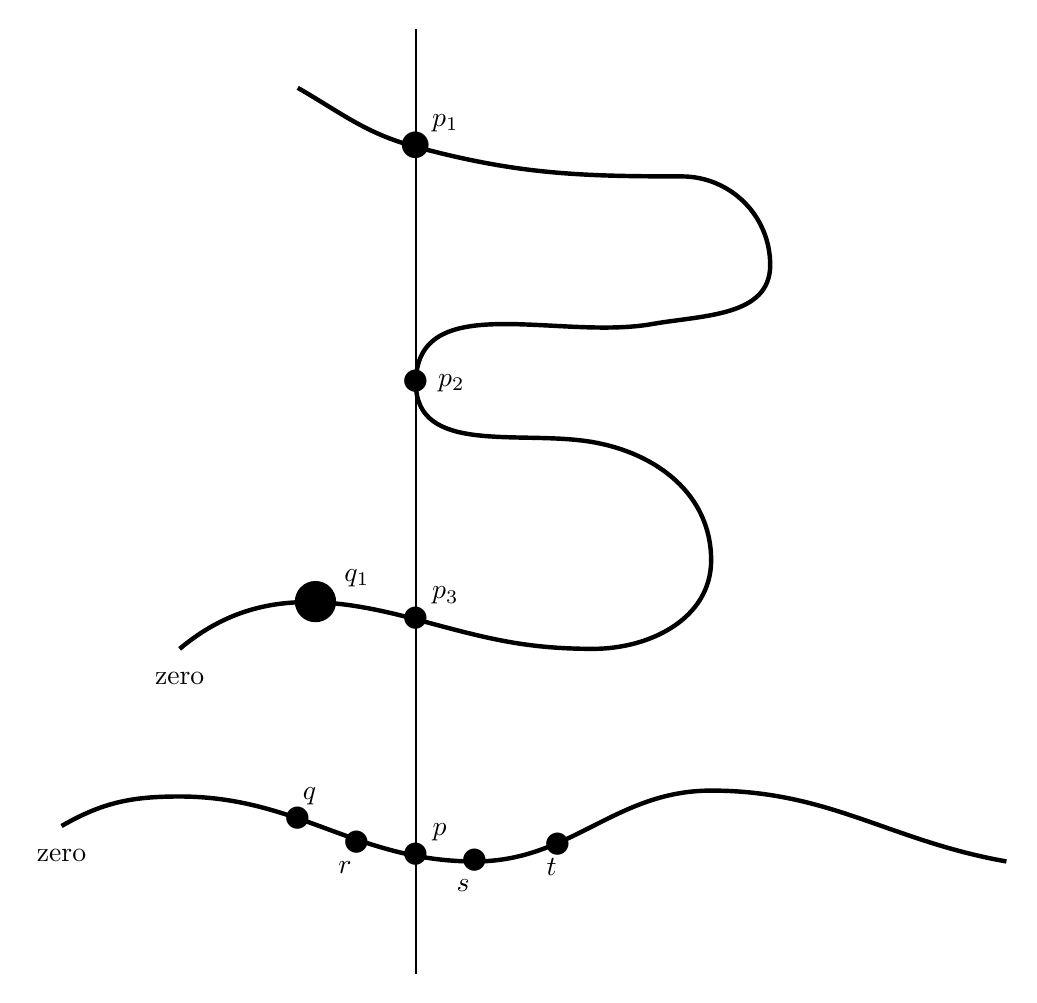
\begin{tikzpicture}[scale = 1.5]

\draw[thick] (0, 0) to (0, 8);

\node at (-3, 1) {zero};

\node at (0, 1) {\huge $\bullet$};
\node at (.2, 1.2) {$p$};

\node at (-1, 1.3) {\huge $\bullet$};
\node at (-.9, 1.5) {$q$};

\node at (-2, 2.5) {zero};

\draw [fill] (-.85, 3.15) circle [radius = .17];
\node at (-.5, 3.35) {$q_1$};

\node at (-.5, 1.1) {\huge $\bullet$};
\node at (-.6, .9) {$r$};

\node at (.5, .95) {\huge $\bullet$};
\node at (.4, .75) {$s$};

\node at (1.2, 1.08) {\huge $\bullet$};
\node at (1.15, .9) {$t$};

\node at (0, 3) {\huge $\bullet$};
\node at (.25, 3.2) {$p_3$};

\node at (0, 5) {\huge $\bullet$};
\node at (.3, 5) {$p_2$};

\node at (0, 7) {\Huge $\bullet$};
\node at (.25, 7.2) {$p_1$};

\draw[ultra thick] (-3, 1.25) to [out = 30, in = 180] (-2, 1.5) to [out = 0, in = 180] (.5, .95) to [out = 0, in = 180] (2.5, 1.55) to [out = 0, in = 170] (5, .95);

\draw[ultra thick] (-2, 2.75) to [out = 40, in = 165] (0, 3) to [out = -15, in = 180] (1.5, 2.75) to [out = 0, in = -90] (2.5, 3.5) to [out = 90, in = -10] (1.5, 4.5) to [out = 170, in = -90] (0, 5) to [out = 90, in = 190] (2, 5.5) to [out = 10, in = -90] (3, 6) to [out = 90, in = 0] (2.25, 6.75) to [out = 180, in = -15] (0, 7) to [out = 165, in = -30] (-1, 7.5);

\end{tikzpicture}
$$
\caption{Diagram of $\Spec(\sO_K) \rightarrow \Spec(\ZZ)$}
\label{fig:O_KoverSpecZ}
\end{figure}


\section{A Method for Factoring Primes that Often Works}

Suppose $a\in\sO_K$ is such that $K=\QQ(a)$, and let $f(x) \in \ZZ[x]$
be the minimal polynomial of~$a$. Then $\ZZ[a]\subset \sO_K$, and
we have a diagram of schemes
$$
  \begin{tikzcd}
    \displaystyle\bigcup\Spec\left(\sO_K/\p_i^{e_i}\right) \ar[r,hook] \ar[d] & \Spec(\sO_K) \ar[d]
    \\
    \displaystyle\bigcup\Spec\left(\FF_p[x]/(\overline{f}_i^{e_i})\right) \ar[r,hook] \ar[d] & \Spec(\ZZ[a]) \ar[d]
    \\
    \Spec(\FF_p) \ar[r,hook] & \Spec(\ZZ)
  \end{tikzcd}
$$

where $\overline{f} = \prod_i \overline{f}_i^{e_i}$ is the factorization of the
image of $f$ in $\FF_p[x]$, and $p\sO_K = \prod \p_i^{e_i}$ is the factorization
of $p\sO_K$ in terms of prime ideals of $\sO_K$. On the level of rings, the
bottom horizontal map is the quotient map $\ZZ\to\ZZ/p\ZZ\isom \FF_p$.
The middle horizontal map is induced by
$$
  \ZZ[x] \to \bigoplus_i \FF_p[x]/(\overline{f}_i^{e_i}),
$$
and the top horizontal map is induced by
$$
  \sO_K \to \sO_K/p\sO_K \isom \bigoplus \sO_K/\p_i^{e_i},
$$
where the isomorphism is by the Chinese Remainder Theorem,
which is Theorem~\ref{thm:crt} below.
The left vertical maps come from the inclusions
$$
   \FF_p \hookrightarrow \FF_p[x]/(\overline{f}_i^{e_i}) \hookrightarrow \sO_K/\p_i^{e_i},
$$
and the right from the inclusions $\ZZ \hookrightarrow \ZZ[a] \hookrightarrow \sO_K$.

The cover $\pi:\Spec(\ZZ[a]) \rightarrow \Spec(\ZZ)$ is easy to understand because it is
defined by the single equation $f(x)$,
in the sense that $\ZZ[a] \isom \ZZ[x]/(f(x))$.
To give a maximal ideal~$\p$ of $\ZZ[a]$ such that $\pi(\p) = p\ZZ$ is the same
as giving a homomorphism $\varphi: \ZZ[x]/(f) \rightarrow \overline{\FF}_p$ up to automorphisms of
the image, which is in turn the same as giving a root of~$f$ in $\overline{\FF}_p$ up
to automorphism, which is the same as giving an irreducible factor of the
reduction of~$f$ modulo~$p$.

\begin{lemma}\ilem{factorization of $p\sO_K$}\label{lem:factpok}
  Suppose the index of $\ZZ[a]$ in $\sO_K$ is coprime to~$p$.
  Then the primes~$\p_i$ in the factorization of $p\ZZ[a]$ do not
  decompose further going from $\ZZ[a]$ to $\sO_K$, so finding the
  prime ideals of $\ZZ[a]$ that contain~$p$ yields the primes
  that appear in the factorization of $p\sO_K$.
\end{lemma}
\begin{proof}
  % {\em Low-brow argument:}
  Fix a basis for $\sO_K$ and for $\ZZ[a]$ as $\ZZ$-modules.
  Form the matrix~$A$ whose columns express each basis element
  of $\ZZ[a]$ as a $\ZZ$-linear combination of the basis for $\sO_K$.
  Then
  $$
    \det(A) = \pm [\sO_K:\ZZ[a]]
  $$
  is coprime to~$p$, by hypothesis. Thus the reduction of~$A$
  modulo~$p$ is invertible, so it defines an isomorphism
  $\ZZ[a]/p\ZZ[a] \isom \sO_K/p\sO_K$.

  Let $\overline{\FF}_p$ denote a fixed algebraic closure of $\FF_p$; thus $\overline{\FF}_p$
  is an algebraically closed field of characteristic~$p$, over which
  all polynomials in $\FF_p[x]$ factor into linear factors.
  Any homomorphism $\sO_K\to \overline{\FF}_p$ sends~$p$ to~$0$, so is the composition
  of a homomorphism $\sO_K \to \sO_K/p\sO_K$ with a homomorphism
  $\sO_K/p\sO_K \to \overline{\FF}_p$. Since $\sO_K/p\sO_K \isom \ZZ[a]/p\ZZ[a]$, the
  homomorphisms $\sO_K\to \overline{\FF}_p$ are in bijection with the homomorphisms
  $\ZZ[a]\to \overline{\FF}_p$. The homomorphisms $\ZZ[a]\to\overline{\FF}_p$ are in bijection
  with the roots of the reduction modulo~$p$ of the minimal polynomial
  of~$a$ in $\overline{\FF}_p$.
\end{proof}

\begin{remark}
  Here is a ``high-brow'' proof of Lemma~\ref{lem:factpok}.
  By hypothesis we have an exact sequence of abelian groups
  $$
    0 \to \ZZ[a] \to \sO_K \to H \to 0,
  $$
  where $H$ is a finite abelian group of order coprime to~$p$.
  Tensor product is right exact, and there is an exact sequence
  $$
     \Tor_1(H,\FF_p) \to \ZZ[a]\otimes\FF_p \to \sO_K\otimes\FF_p \to H\otimes\FF_p \to 0,
  $$
  and $\Tor_1(H,\FF_p) = 0$ (since $H$ has no $p$-torsion),
  so $\ZZ[a]\otimes\FF_p \isom \sO_K\otimes\FF_p$.
\end{remark}

As suggested in the proof of the lemma, we find all homomorphisms
$\sO_K\to \overline{\FF}_p$ by finding all homomorphism
$\ZZ[a] \to \overline{\FF}_p$.  In
terms of ideals, if $\p = (f(a),p)\ZZ[a]$ is a maximal ideal of $\ZZ[a]$,
then the ideal $\p' = (f(a),p)\sO_K$ of $\sO_K$ is also maximal, since
$$
  \sO_K/\p'\isom (\sO_K/p\sO_K)/(f(\tilde{a}))
  \isom
  (\ZZ[a]/p\ZZ[a]) / (f(\tilde{a})) \subset \overline{\FF}_p,
$$
where $\tilde{a}$ denotes the image of $a$ in $\sO_K/p\sO_K$.

We formalize the above discussion, together with
Exercise~\ref{exercise:ramification-for-prime-factoring-easy-way} below,
in the following theorem:
\begin{theorem}\label{thm:fac1}\ithm{prime ideal factorization}
  Let $f\in\ZZ[x]$ be the minimal polynomial of~$a$ over~$\ZZ$.
  Suppose that~$p\nmid [\sO_K:\ZZ[a]]$ is a prime. Let
  $$
    \overline{f} = \prod_{i=1}^t \overline{f}_i^{e_i} \in \FF_p[x]
  $$
  where the $\overline{f}_i$ are distinct monic irreducible
  polynomials. Let $\p_i = (p,f_i(a))$ where $f_i\in\ZZ[x]$ is a
  lift of $\overline{f}_i$ in $\FF_p[x]$. Then
  $$
    p\sO_K = \prod_{i=1}^t \p_i^{e_i}.
  $$
  %Geometrically, the fiber of $\Spec(\sO_K) \to p\ZZ$
  %contains the points $\{\p_1,\p_2,\ldots, \p_t\}$
  %with multiplicites $e_i$.
\end{theorem}

\begin{exercise}\label{exercise:ramification-for-prime-factoring-easy-way}
  Let $p$ be a prime. Let $\sO_K$ be the ring of integers of a number
  field $K$, and suppose that $a\in \sO_K$ is such that $[\sO_K:\ZZ[a]]$ is
  finite and coprime to~$p$. Let $f(x)$ be the minimal polynomial of~$a$.
  We have already shows that if the reduction $\overline{f}\in\FF_p[x]$ of $f$
  factors as
  $$
    \overline{f} = \prod g_i^{e_i},
  $$
  where the $g_i$ are distinct irreducible polynomials in $\FF_p[x]$,
  then the primes appearing in the factorization of $p\sO_K$ are the
  ideals $(p,g_i(a))$. Show that the exponents of the primes in the
  factorization of $p\sO_K$ are the $e_i$.
\end{exercise}


We return to the example from above, in which $K = \QQ(a)$, where~$a$ is
a root of $f = x^5 + 7x^4 + 3x^2 - x + 1$.  The ring of integers~$\sO_K$
has discriminant $2945785 = 5\cdot 353\cdot 1669$, as the following
{\Sage} code shows.
\begin{sagecode}
\begin{sagecell}
K.<a> = NumberField(x^5 + 7*x^4 + 3*x^2 - x + 1)
D = K.discriminant(); D
\end{sagecell}
\begin{sageout}
2945785
\end{sageout}
\begin{sagecell}
factor(D)
\end{sagecell}
\begin{sageout}
5 * 353 * 1669
\end{sageout}
\end{sagecode}
The order $\ZZ[a]$ has the same discriminant as $f(x)$, which
is the same as the discriminant of $\sO_K$, so
$\ZZ[a] = \sO_K$ and we can apply the above theorem.
(Here we use that the index of $\ZZ[a]$ in $\sO_K$
is the square of the quotient of their discriminants,
a fact we will prove later in Section~\ref{sec:disc}.)
\begin{sagecode}
\begin{sagecell}
R.<x> = QQ[]
discriminant(x^5 + 7*x^4 + 3*x^2 - x + 1)
\end{sagecell}
\begin{sageout}
2945785
\end{sageout}
\end{sagecode}
We have
$$
  x^5+7x^4+3x^2-x+1 \equiv (x+2) \cdot (x+3)^2 \cdot (x^2+4x+2)\pmod{5},
$$
which yields the factorization of $5\sO_K$ given before the theorem.

If we replace $a$ by $b = 7a$, then the index of $\ZZ[b]$
in $\sO_K$ will be a power of $7$, which is coprime to $5$,
so the above method will still work.
\begin{sagecode}
\begin{sagecell}
K.<a> = NumberField(x^5 + 7*x^4 + 3*x^2 - x + 1)
f = (7*a).minpoly('x')
f
\end{sagecell}
\begin{sageout}
x^5 + 49*x^4 + 1029*x^2 - 2401*x + 16807
\end{sageout}
\begin{sagecell}
f.disc()
\end{sagecell}
\begin{sageout}
235050861175510968365785
\end{sageout}
\begin{sagecell}
factor(f.disc() / K.disc())
\end{sagecell}
\begin{sageout}
7^20
\end{sageout}
\begin{sagecell}
f.factor_mod(5)
\end{sagecell}
\begin{sageout}
(x + 4) * (x + 1)^2 * (x^2 + 3*x + 3)
\end{sageout}
\end{sagecode}
Thus $5$ factors in $\sO_K$
as
$$
  5\sO_K = (5, 7a+1)^2 \cdot (5, 7a+4) \cdot (5, (7a)^2 + 3(7a) + 3).
$$
If we replace $a$ by $b=5a$ and try the above algorithm with $\ZZ[b]$, then
the method fails because the index of $\ZZ[b]$ in $\sO_K$ is divisible by~$5$.
\begin{sagecode}
\begin{sagecell}
K.<a> = NumberField(x^5 + 7*x^4 + 3*x^2 - x + 1)
f = (5*a).minpoly('x')
f
\end{sagecell}
\begin{sageout}
x^5 + 35*x^4 + 375*x^2 - 625*x + 3125
\end{sageout}
\begin{sagecell}
f.factor_mod(5)
\end{sagecell}
\begin{sageout}
x^5
\end{sageout}
\end{sagecode}

\section{A General Method}

There are numbers fields $K$ such that $\sO_K$ is not of the form
$\ZZ[a]$ for any $a\in K$.  Even worse, Dedekind found a
field~$K$ such that $2\mid [\sO_K : \ZZ[a]]$ for {\em all}
$a\in \sO_K$, so there is no choice of $a$ such that Theorem~\ref{thm:fac1}
can be used to factor~$2$ for $K$ (see Example~\ref{ex:dedekind} below).

\subsection{Inessential Discriminant Divisors}

\begin{definition}
  A prime $p$ is an \defn{inessential discriminant divisor}
  if $p\mid [\sO_K : \ZZ[a]]$ for {\em every} $a\in\sO_K$.
\end{definition}
See Example~\ref{ex:exdim} below for why it is called an
inessential ``discriminant divisor'' instead of an
inessential ``index divisor''.

Since $[\sO_K : \ZZ[a]]^2$ is the absolute value of
$\Disc(f(x))/\Disc(\sO_K)$, where $f(x)$ is the characteristic
polynomial of $f(x)$, an inessential discriminant divisor divides the
discriminant of the characteristic polynomial of any element of
$\sO_K$.

\begin{example}[Dedekind]\label{ex:dedekind}
  Let $K=\QQ(a)$ be the cubic field defined by a root $a$ of the polynomial
  $f = x^3 + x^2 - 2x+8$.  We will use {\Sage} to show that~$2$ is an
  inessential discriminant divisor for~$K$.
\begin{sagecode}
\begin{sagecell}
K.<a> = NumberField(x^3 + x^2 - 2*x + 8); K
\end{sagecell}
\begin{sageout}
Number Field in a with defining polynomial x^3 + x^2 - 2*x + 8
\end{sageout}
\begin{sagecell}
K.factor(2)
\end{sagecell}
\begin{sageout}
(Fractional ideal (1/2*a^2 - 1/2*a + 1)) * \
(Fractional ideal (-a^2 + 2*a - 3)) * \
(Fractional ideal (-3/2*a^2 + 5/2*a - 4))
\end{sageout}
\end{sagecode}
  Thus $2\sO_K = \p_1\p_2\p_3$, with the $\p_i$ distinct,
  and one sees directly from the above expressions
  that $\sO_K/\p_i \isom \FF_2$ for each $i$. If $\sO_K = \ZZ[a]$
  for some $a \in \sO_K$ with minimal polynomial~$f$, then
  $\overline{f}(x) \in \FF_2[x]$ must be a product of three {\em distinct}
  linear factors, which is impossible, since the only
  linear polynomials in $\FF_2[x]$ are $x$ and $x+1$.
\end{example}

\begin{exercise}
  Find an example of a field $K$ of degree at least~$4$ such that the ring
  $\sO_K$ of integers of $K$ is not of the form $\ZZ[a]$ for any $a\in \sO_K$.
\end{exercise}

\begin{exercise}
  Let $\p$ be a prime ideal of $\sO_K$, and suppose that $\sO_K/\p$
  is a finite field of characteristic $p\in\ZZ$.  Prove that there is
  an element $\alpha\in\sO_K$ such that $\p=(p,\alpha)$.  This
  justifies why we can represent prime ideals of $\sO_K$ as pairs
  $(p,\alpha)$, as is done in {\Sage}. (More generally, if $I$ is an
  ideal of $\sO_K$, we can choose one of the elements of $I$ to be {\em
  any} nonzero element of $I$.)
\end{exercise}

\begin{exercise}
  Give an example of an order $\sO$ in the ring of integers of
  a number field and an ideal $I$ such that~$I$ cannot be generated by
  $2$ elements as an ideal.

  \begin{hint}
    This problem is more difficult than usual.
  \end{hint}
\end{exercise}

\subsection{Remarks on Ideal Factorization in General}

Recall (from Definition~\ref{defn:order}) that an {\em order} in $\sO_K$ is
a subring $\sO$ of $\sO_K$ that has finite index in $\sO_K$.  For
example, if $\sO_K = \ZZ[i]$, then $\sO = \ZZ + 5\ZZ[i]$ is an order in $\sO_K$,
and as an abelian group $\sO_K/\sO$ is cyclic of order~$5$.

Most algebraic number theory books do not describe an algorithm for
decomposing primes in the general case.  Fortunately, Cohen's book
\cite[Ch.~6]{cohen:course_ant} does describe how to solve the general
problem, in more than one way.  The algorithms are nontrivial, and
occupy a substantial part of Chapter~6 of Cohen's book.  Our goal
for the rest of this section is to give a hint as to what goes into them.

The general solutions to prime ideal factorization are somewhat surprising,
since the algorithms are much more sophisticated than the one
suggested by Theorem~\ref{thm:fac1}.  However, these complicated
algorithms all run very quickly in practice, even without assuming the
maximal order is already known.  In fact, they avoid computing~$\sO_K$
altogether, and instead compute only an order~$\sO$ that is {\em $p$-maximal},
i.e., is such that $p \nmid [\sO_K:\sO]$.

For simplicity we consider the following slightly easier problem whose
solution illustrates the key ideas needed in the general case.
\begin{problem}\label{prob:pcontained}
  Let $\sO$ be any order in $\sO_K$ and let~$p$ be a prime of $\ZZ$.
  Find the prime ideals of $\sO$ that contain~$p$.
\end{problem}

Given a prime~$p$
that we wish to factor in $\sO_K$, we first find a $p$-maximal order~$\sO$.
We then use a solution to Problem~\ref{prob:pcontained} to find
the prime ideals $\p$ of $\sO$ that contain $p$.  Second, we find
the exponents $e$ such that $\p^e$ exactly divides $p\sO$.
The resulting factorization in $\sO$ completely determines
the factorization of $p\sO_K$.

A $p$-maximal order can be found reasonably quickly in practice using
algorithms called ``round 2'' and ``round 4''.  To
compute $\sO_K$, given an order $\ZZ[\alpha]\subset \sO_K$, one takes a
sum of $p$-maximal orders, one for every~$p$ such that $p^2$ divides
$\Disc(\ZZ[\alpha])$.  The time-consuming part of this computation is
finding the primes~$p$ such that $p^2\mid \Disc(\ZZ[\alpha])$, not
finding the $p$-maximal orders.  This example illustrates that
a fast algorithm for factoring integers would not only break the RSA
cryptosystems, but would massively speed up computation of the ring of
integers of a number field.
\begin{remark}
  The MathSciNet review of \cite{buchmann_lenstra:approx} by
  J.~Buhler contains the following:
  \begin{quote}
      A result of Chistov says that finding the ring of integers $\sO_K$
      in an algebraic number field $K$ is equivalent, under certain
      polynomial time reductions, to the problem of finding the largest
      squarefree divisor of a positive integer. No feasible (i.e.,
      polynomial time) algorithm is known for the latter problem, and it
      is possible that it is no easier than the more general problem of
      factoring integers.
  \end{quote}
  Thus it appears that computing the ring $\sO_K$ is quite hard.
\end{remark}

\subsection{Finding a $p$-Maximal Order}\label{sec:alg_pmax}

Before describing the general factorization algorithm, we sketch some
of the theory behind the general algorithms for computing a
$p$-maximal order $\sO$ in $\sO_K$.  The main input is the following theorem:
\begin{theorem}[Pohst-Zassenhaus]
  Let $\sO$ be an order in the ring of integers $\sO_K$ of a number field,
  let $p\in\ZZ$ be a prime, and let
  $$
    I_p = \{x \in \sO : x^m \in p\sO \text{ for some $m\geq 1$}\} \subset \sO
  $$
  be the radical of $p\sO$, which is an ideal of $\sO$. Let
  $$
    \sO' = \{x \in K : xI_p \subset I_p\}.
  $$
  Then $\sO'$ is an order and either $\sO'=\sO$, in which case $\sO$ is
  $p$-maximal, or $\sO\subset\sO'$ and $p$ divides $[\sO':\sO]$.
\end{theorem}
\begin{proof}
  We prove here only that $[\sO':\sO] \mid p^n$, where $n$ is the degree
  of $K$.  We have $p\in I_p$, so if $x \in \sO'$, then $xp \in
  I_p\subset \sO$, which implies that $x\in \frac{1}{p}\sO$.  Since
  $(\frac{1}{p}\sO)/\sO$ is of order $p^n$, the claim follows.

  To complete the proof, we would show that if $\sO' = \sO$, then $\sO$ is
  already $p$-maximal.  See \cite[\S6.1.1]{cohen:course_ant} for the
  rest if this proof.
\end{proof}

After deciding on how to represent elements of~$K$ and orders and
ideals in~$K$, one can give an efficient algorithm to compute the
$\sO'$ of the theorem.  The algorithm mainly involves linear algebra
over finite fields.  It is complicated to describe, but efficient in
practice, and is conceptually simple---just compute~$\sO'$.  The trick
for reducing the computation of $\sO'$ to linear algebra is the
following lemma:
\begin{lemma}
  Define a homomorphism $\psi:\sO \hookrightarrow \End(I_p/ p I_p)$ given by
  sending $\alpha\in\sO$ to left multiplication by the reduction of
  $\alpha$ modulo~$p$.  Then
  $$
    \sO'=\frac{1}{p} \ker(\psi).
  $$
\end{lemma}
\begin{proof}
  If $x \in \sO'$, then $x I_p \subset I_P$, so $\psi(x)$ is the $0$
  endomorphism.  Conversely, if $\psi(x)$ acts as $0$ on $I_p/ p I_p$,
  then clearly $x I_p \subset I_p$.
\end{proof}

Note that to give an algorithm one must also figure out how to
explicitly compute $I_p/ p I_p$ and the kernel of this map
(see  the next section for more
details).

\subsection{General Factorization Algorithm of Buchman-Lenstra}

We finally give an algorithm to factor $p\sO_K$ in general. This is a
summary of the algorithm described in more detail in
\cite[\S6.2]{cohen:course_ant}.

\begin{algorithm}[Factoring a Finite Separable Algebra]\label{alg:factorsep}
  Let $A$ be a finite separable algebra over $\FF_p$.  This
  algorithm either shows that $A$ is a field or finds
  a nontrivial idempotent in $A$, i.e., an $\varepsilon\in A$
  such that $\varepsilon^2 = \varepsilon$ with $\varepsilon\neq 0$ and $\varepsilon\neq 1$.
  \begin{enumerate}
    \item The dimension of the kernel $V$ of the map $x\mapsto x^p - x$ is
    equal to $k$.  This is because abstractly we have that $A\ncisom
    A_1\times \cdots \times A_k$, with each $A_i$ a finite field
    extension of $\FF_p$.
    \item If $k=1$ we are done.  Terminate.
    \item Otherwise, choose $\alpha \in V$ with $\alpha \not\in \FF_p$.
    (Think of $\FF_p$ as the diagonal embedding of $\FF_p$ in
    $A_1\times \cdots \times A_k$).
    Compute powers of $\alpha$ and find the minimal polynomial $m(X)$
    of $\alpha$.
    \item Since $V\ncisom \FF_p \times \cdots \times F_p$ ($k$ factors),
    the polynomial $m(X)$ is a square-free product of linear factors, that
    has degree $>1$ since $\alpha\not\in\FF_p$.  Thus we can compute
    a splitting $m(X) = m_1(X) \cdot m_2(X)$, where both $m_i(X)$ have
    positive degree.
    \item Use the Euclidean algorithm in $\FF_p[X]$ to find
    $U_1(X)$ and $U_2(X)$ such that
    $$
      U_1 m_1 + U_2 m_2 = 1.
    $$
    \item Let $\varepsilon = (U_1 m_1)(\alpha)$.  Then we have
    $$
      U_1 m_1 U_1 m_1 + U_2 m_2 U_1 m_1 = U_1 m_1,
    $$
    so since $(m_1 m_2)(\alpha) = m(\alpha)=01$, we have $\varepsilon^2 = \varepsilon$.
    Also, since $\gcd(U_1, m_2) = \gcd(U_2, m_1) = 1$,
    we have $\varepsilon\neq 0$ and $\varepsilon \neq 1$.
  \end{enumerate}
\end{algorithm}

Given Algorithm~\ref{alg:factorsep}, we compute an idempotent
$\varepsilon \in A$, and observe that
$$
  A \isom \ker(1 - \varepsilon)  \oplus \ker(\varepsilon).
$$
Since $(1 - \varepsilon) + \varepsilon = 1$, we see that
$(1 - \varepsilon)v + \varepsilon v = v$, so that the sum
of the two kernels equals $A$.
Also, if $v$ is in the intersection of the two kernels,
then $\varepsilon(v) = 0$ and $(1-\varepsilon)(v) =0$, so
$0 = (1-\varepsilon)(v) = v - \varepsilon(v) = v$, so the sum is direct.

\begin{remark}
  The beginning of \cite[\S6.2.4]{cohen:course_ant} suggests that one
  can just randomly find an $\alpha \in A$ such that $A\isom
  \FF_p[x]/(m(x))$ where $m$ is the minimal polynomial of $\alpha$.
  This is usually the case, but is {\em wrong in general}, since there
  need {\em not} be an $\alpha \in A$ such that $A \isom
  \FF_p[\alpha]$.  For example, let $p=2$ and $K$ be as in
  Example~\ref{ex:dedekind}.  Then $A \isom \FF_2 \times \FF_2 \times
  \FF_2$, which as a ring is not generated by a single element, since
  there are only 2 distinct linear polynomials over $\FF_2[x]$.
\end{remark}

\begin{algorithm}[Factoring a General Prime Ideal]\label{alg:genfac}
  Let $K=\QQ(a)$ be a number field given by an algebraic integer~$a$
  as a root of its minimal monic polynomial~$f$ of degree~$n$.
  We assume that an order $\sO$ has been given by a basis $w_1,\ldots,w_n$
  and that~$\sO$ that contains $\ZZ[a]$.
  For any prime $p\in\ZZ$, the following algorithm computes the set of
  maximal ideals of~$\sO$ that contain~$p$.
  \begin{description}
    \item[\normalfont (Check if easy):] If $p \nmid \Disc(\ZZ[a]) / \Disc(\sO)$ (so
    $p \nmid [\sO:\ZZ[a]]$), then using Theorem~\ref{thm:fac1} we
    factor~$p\sO$.

    \item[\normalfont (Compute radical):]
    Let $I$ be the \defn{radical} of $p\sO$, which is the ideal of
    elements $x\in\sO$ such that $x^m\in p\sO$
    for some positive integer~$m$.  Note that $p\sO \subset I$, i.e.,
    $I\mid p\sO$; also~$I$ is the product
    of the primes that divide $p$, without multiplicity.
    Using linear algebra over the finite field
    $\FF_p$, we compute a basis for $I/p\sO$ by computing
    the abelian subgroup of $\sO/p\sO$ of all nilpotent
    elements.  This computes $I$, since $p\sO\subset I$.

    \item[\normalfont (Compute quotient by radical):]
    Compute an $\FF_p$ basis for
    $$
      A = \sO/I = (\sO/p\sO)/(I/p\sO).
    $$
    The second equality comes from the fact that $p\sO\subset I$.
    Note that $\sO/p\sO$
    is obtained by simply reducing the basis $w_1,\ldots, w_n$ modulo~$p$.
    Thus this step entirely involves linear algebra modulo $p$.

    \item[\normalfont (Decompose quotient):] The ring $A$ is isomorphic to
    the quotient of $\sO$ by a radical ideal,
    so it decomposes as a product
    $A \isom A_1 \times \cdots \times A_k$ of finite fields.
    We find such a decomposition explicitly using Algorithm~\ref{alg:factorsep}.

    \item[\normalfont (Compute the maximal ideals over $p$):] Each maximal ideal
    $\p_i$ lying over~$p$ is the kernel of one of the compositions
    $$
      \sO \to A \ncisom A_1 \times \cdots \times A_k \to A_i.
    $$
  \end{description}
\end{algorithm}
Algorithm~\ref{alg:genfac} finds all primes of $\sO$ that contain the radical $I$ of
$p\sO$.  Every such prime clearly contains $p$, so to see that the
algorithm is correct, we prove that the primes $\p$ of $\sO$ that
contain~$p$ also contain~$I$.  If $\p$ is a prime of $\sO$ that
contains~$p$, then $p\sO \subset \p$.  If $x\in I$ then $x^m\in p\sO$
for some $m$, so $x^m\in \p$ which implies that $x\in \p$ by the primality
of $\p$.  Thus $\p$ contains $I$, as required.  Note that we do not find the powers of
primes that divide $p$ in Algorithm~\ref{alg:genfac}; that's left to another
algorithm that we will not discuss in this book.

Algorithm~\ref{alg:genfac} was invented by J.~Buchmann and
H.W. Lenstra, though their paper seems to have never been
published; however, the algorithm is described in detail in
\cite[\S6.2.5]{cohen:course_ant}.  Incidentally, this chapter is based
on Chapters~4 and~6 of \cite{cohen:course_ant}, which is highly
recommended, and goes into much more detail about these algorithms.

\begin{exercise}
  Explicitly factor the ideals generated by each of $2$, $3$, and $5$ in
  the ring of integers of $\QQ(\sqrt[3]{2})$ (so you will factor $3$
  separate ideals as products of prime ideals.)
  You may assume that the ring of integers of $\QQ(\sqrt[3]{2})$
  is $\ZZ[\sqrt[3]{2}]$, but do \em{not} simply use a computer command to do
  the factorizations.
\end{exercise}

\begin{exercise}
  Let $K=\QQ(\zeta_{13})$,where $\zeta_{13}$ is a primitive $13$th root of
  unity. Note that~$K$ has ring of integers $\sO_K=\ZZ[\zeta_{13}]$.
  \begin{enumerate}
    \item Factor $2$, $3$, $5$, $7$, $11$, and $13$ in the ring
    of integers $\sO_K$.  You may use a computer.
    \item For $p\neq 13$, find a conjectural
    relationship between the number of prime ideal factors of $p\sO_K$
    and the order of the reduction of~$p$  in $(\ZZ/13\ZZ)^*$.
    \item Compute the minimal polynomial $f(x)\in\ZZ[x]$ of $\zeta_{13}$.
    Reinterpret your conjecture as a conjecture that
    relates the degrees of the irreducible factors of $f(x)\pmod{p}$ to
    the order of $p$ modulo~$13$. Does your conjecture
    remind you of quadratic reciprocity?
  \end{enumerate}
\end{exercise}

%%[[Add discussion about how to compute a $p$-maximal order here.]]
